\section{Analysis}
\subsection{Introduction}

The Clinic of Masticatory Disorders of the Zurich University treats among other facial pain and mandibular joint problems. For better diagnosis the Clinic has developed an own 3D camera system, \gls{optis} to record the mastication movement of the patient. The 3D cameras record the position of 2 triangles of 3 LEDs each, triangles fixed to the patient's mandibular.


\begin{figure}[h!]
	\centering
	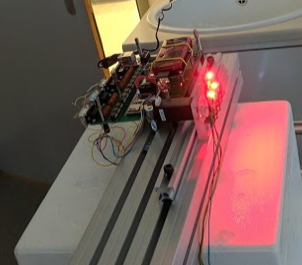
\includegraphics[width=0.3\textwidth]{leds}
	\caption{LED triangle example of the Optis system }
\end{figure}

\noindent One triangle is fix (static) in the upper jaw, while the second moves with the mandible. This movement is recorded by Optis in form of coordinates and saved to \glspl{gls-MVM} (MVM) files, also a proprietary file extension.

\begin{figure}[h!]
	\centering
	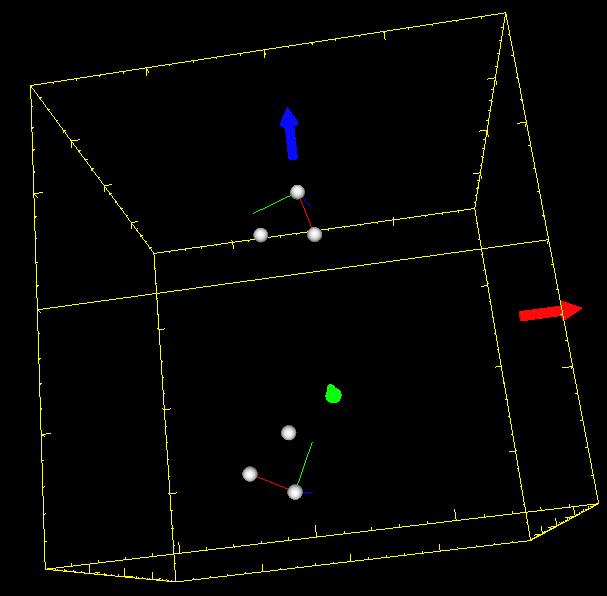
\includegraphics[width=0.4\textwidth]{optis_leds}
	\caption{LEDs triangles in Optis application}
\end{figure}



\begin{wrapfigure}{r}{0.4\textwidth}
\begin{center}
	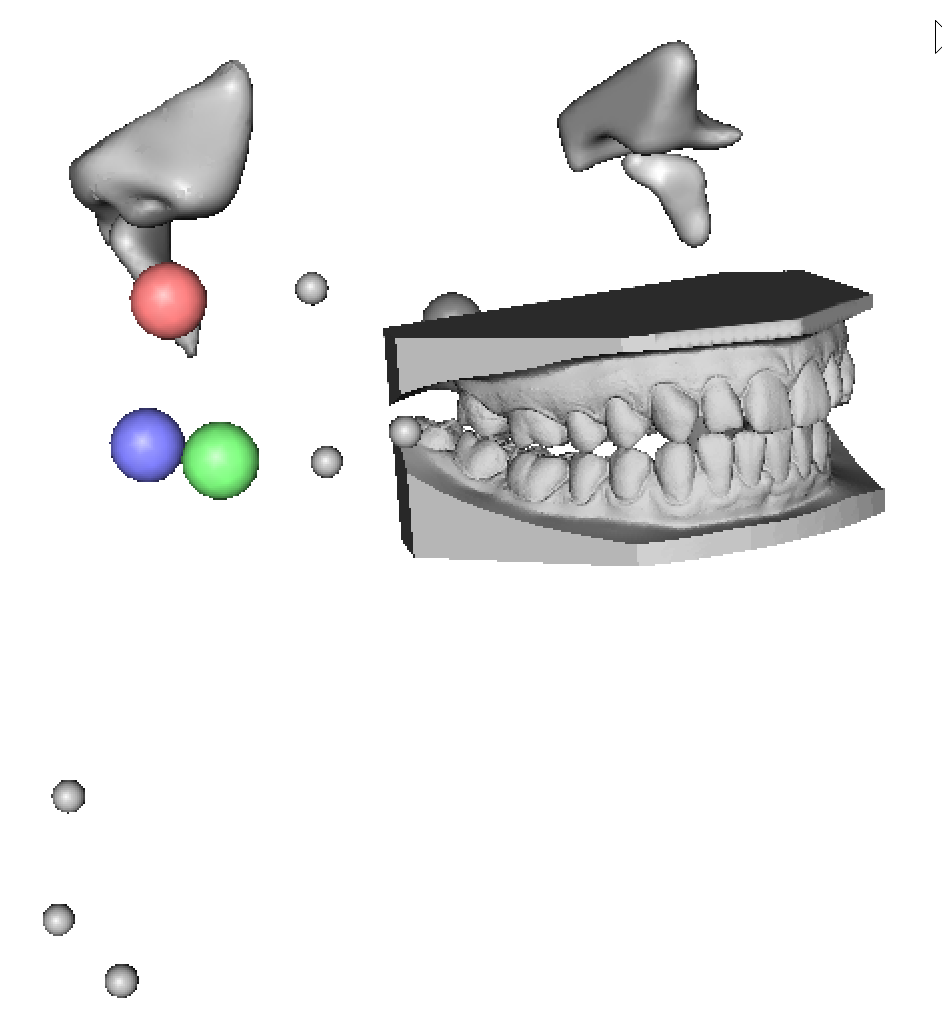
\includegraphics[width=0.3\textwidth]{tmjviewer}
	\caption{TMJViewer}
\end{center}
\end{wrapfigure}
The jaw movement is only one piece of the system. The another piece are the MRI images of the patient. These are stored in form of \gls{gls-STL} (STL) files (or \glspl{anatomy}). Together with the MVM files, another proprietary software of the Clinic, \gls{tmjviewer}, can display the movement applied to the patient's anatomy. So the doctors can elaborate a diagnosis.

But the process required to achieve this goal is boring, tedious and above all, error-prone. All required files come from different sources and must be processed with different applications before using them with TeamViewer.

In the course of this project an application capable of importing \gls{STL} files, movement data in form of \gls{MVM} files or a stream, and displaying all of them with animation should be developed. The application should be able to display the movement in real-time or offline modus. The user should be able to choose which elements can be animated.


\subsection{Requirements Specification}
\subsubsection{General Description}
There are two possible application scenarios:
\begin{itemize}
	\item Offline Modus
	\item Real-time Modus
\end{itemize}


\paragraph{Offline Modus:} 
The user has to enter manually all the data, \acrshort{STL} and \acrshort{MVM} files and other parameters needed by the application and configure it. The application can replay the movement any number of times.
\paragraph{Real-Time Modus:} 
The user has to enter only the \acrshort{STL} and the network parameters needed to connect the application with the 3D cameras via socket. The application can record the real-time movement and replay it.\footnote{Due to missing information from the project partner it was not possible to develop the Real-Time Modus. Explanations follow.} 

\subsubsection{Functional Requirements} \label{fr:1}
\begin{table}[h!] 
	\begin{center}
		\begin{tabular}{ p{0.6cm}||p{3.5cm}|p{9cm}|p{1.1cm} }\beforeheading
			\heading{\textbf{ID}} & \heading{\textbf{Name} } & \heading{\textbf{Description}	}                                              & \heading{\textbf{Priority}}\\\afterheading
			FR1  			      & Load anatomy             & The application imports one or more graphic anatomy objects           		    & $\star \star \star $ 		\\\normalline
			FR2 			      & Load movement            & The application imports objects containing information about movement           & $\star \star \star $		\\\normalline
			FR3 			      & Configuration            & The application supports movements configuration                                & $\star \star \star $		\\\normalline
			FR4                   & Display anatomy          & The application shows the anatomy elements statically                           & $\star \star \star $       \\\normalline
			FR5                   & Display movement         & The application shows the movement of one or more anatomy elements              & $\star \star \star $       \\\normalline
			FR6                   & Real-time movement       & The application shows the movement of one or more anatomy elements in real time & $\star \star \star $      	\\\normalline
			FR7                   & Record movement          & The application is able to record  movement at real-time                        & $\star \star \star $      	\\\normalline
			FR8                   & Select anatomy           & The application supports selection of one or more anatomy elements              & $\star \star  $  			\\\normalline
			FR9                   & Select movement	         & The application the selection of movement objects						       & $\star \star  $            \\\normalline
			FR10                  & Show trajectories        & The application shows the trajectory of a selected moving anatomy element       & $\star  $					\\\normalline
			FR11                  & Color anatomy            & The application supports coloring of one or more anatomy elements               & $\star  $					\\\lastline
		\end{tabular}
		\caption{Functional Requirements}
	\end{center}
\end{table}

\newpage

\subsubsection{Non Functional Requirements}
\paragraph{Technology} \gls{opengl} shall be used for graphics processing
\paragraph{GUI} The application's GUI accomplishes modern standards                             
\paragraph{Frame Rate} The must display the graphics with at least 24 FPS TODO: ask Konrad about this. 
\paragraph{Platform} The application shall run only in Windows, Windows 7 or above
\paragraph{Security}
\begin{itemize}
	\item \textbf{Confidentiality} The application shall not make the patient data available to unauthorized individuals or entities 
	\item \textbf{Availability} The application must facilitate the delivery of patient's data from the doctor to the patient
\end{itemize}
\paragraph{Reliability}
\begin{itemize}
	\item \textbf{Recoverability} After a system crash or abnormal system end the application shall start again without problem. 
\end{itemize}
\paragraph{Usability}
\begin{itemize}
	\item \textbf{Learnability}  A new user should need maximal 10 minutes to learn how to operate with the application.
	\item \textbf{Operability} The application shall be a desktop application only.
\end{itemize}
\paragraph{Installability} The installation of the application should not take more than 2 minutes.
\paragraph{Durability} All user input in the GUI must be validated. Wrong input must be warned, in order to give the user the opportunity of correcting it.

\subsubsection{Use Cases} \label{use-cases}
\textbf{Use Cases Diagram}

\begin{figure}[h!]
	\centering
	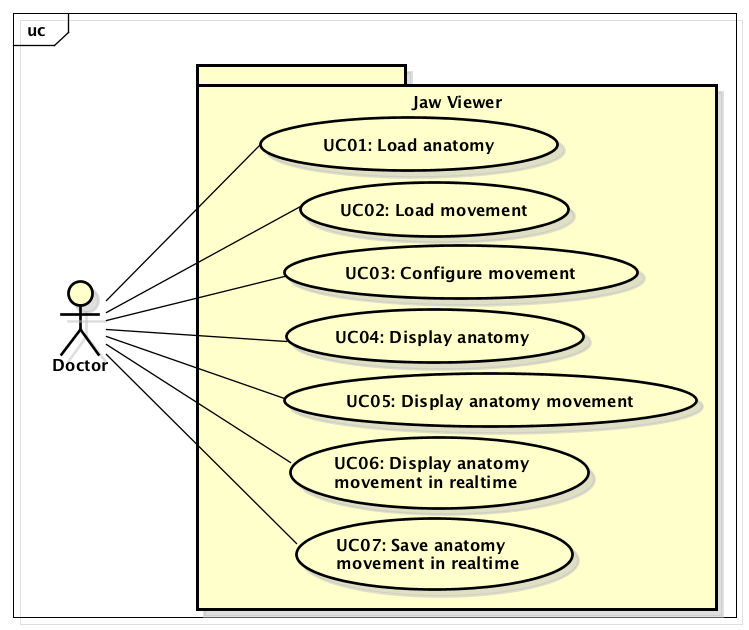
\includegraphics[width=0.6\textwidth]{uc}
	\caption{Use Cases}
\end{figure}

\newpage

\subsubsubsection{Actors}
\begin{table}[!h]
	\begin{tabularx}{\textwidth}{X | X} \beforeheading 
		\heading{Name} & \heading{Description}                                                                                                      \\\afterheading
		Doctor         & An \emph{Doctor} is a member of the medical personal of the Clinic of Masticatory Disorders who uses the \emph{Jaw Viewer}  \\\afterheading 
		Technical Assistant         & An \emph{Technical Assistant} is a non-medical member of the personal of the Clinic of Masticatory Disorders who uses the \emph{Jaw Viewer} \\\lastline
	\end{tabularx}
	\caption{Actors}
\end{table}


\subsubsubsection{UC01: Load anatomy}\label{uc:1}
\begin{table}[!h]
	\begin{tabularx}{\textwidth}{X| X} \beforeheading
		\heading{Mapped Requirement} & \ref{fr:1} FR1, FR8			\\\afterheading                                                   
		\heading{Primary Actor}      & Doctor		\\\afterheading 
		\heading{Story}              & The \emph{Doctor} starts \emph{Jaw Viewer}. The configuration window is shown. The Doctor searches and selects the desired \glspl{anatomy} or \acrshort{STL} files and load them. The files are validated. If they are right they will be displayed as loaded in the configuration window. \\\lastline
	\end{tabularx}
	\caption{UCO1: Load anatomy}
\end{table}

\subsubsubsection{UC02: Load movement} \label{uc:2}
\begin{table}[!h]
	\begin{tabularx}{\textwidth}{X| X} \beforeheading
		\heading{Mapped Requirement} &\ref{fr:1} FR2, FR9			\\\afterheading                                                   
		\heading{Primary Actor}      & Doctor		\\\afterheading 
		\heading{Story}              & After \ref{uc:1} UC01, the configuration window is shown. The Doctor searches and selects the desired movement files or \acrshort{MVM} files and load them. The files are validated. If they are right they will be displayed as loaded in the configuration window. \\\lastline
	\end{tabularx}
	\caption{UCO2: Load movement}
\end{table}


\subsubsubsection{UC03: Configure movement} \label{uc:3}
\begin{table}[!h]
	\begin{tabularx}{\textwidth}{X| X} \beforeheading
		\heading{Mapped Requirement} 	& \ref{fr:1} FR3, FR8, FR9 			\\\afterheading                                                   
		\heading{Primary Actor}  		& Doctor    	\\\afterheading 
		\heading{Story}           	 	& After \ref{uc:1} UC01 and \ref{uc:2} the configuration window is shown to the Doctor. The Doctor can select one or more \acrshort{STL} files and mark them as animated or stationary. The doctor must enter \gls{sphere} and \gls{calibration} parameters. The Doctor can optionally enter network configuration parameters.\\\lastline
	\end{tabularx}
	\caption{UC03: Configure movement}
\end{table}

\newpage

\subsubsubsection{UC04: Display anatomy} \label{uc:4}
\begin{table}[!h]
	\begin{tabularx}{\textwidth}{X| X} \beforeheading
		\heading{Mapped Requirement} & \ref{fr:1} FR4 			\\\afterheading                                                   
		\heading{Primary Actor}      & Doctor		\\\afterheading 
		\heading{Story}              & After \ref{uc:3} UC03, the Doctor starts the visualization and the \glspl{anatomy} are displayed. As only static \acrshort{STL} files were selected, no movement is displayed.  \\\lastline
	\end{tabularx}
	\caption{UC04: Display anatomy}
\end{table}


\subsubsubsection{UC05: Display anatomy movement} \label{uc:5}
\begin{table}[!h]
	\begin{tabularx}{\textwidth}{X| X} \beforeheading
		\heading{Mapped Requirement} & \ref{fr:1} FR5 			\\\afterheading                                                   
		\heading{Primary Actor}      & Doctor		\\\afterheading 
		\heading{Story}              & After \ref{uc:4} UC04, the Doctor starts the visualization and the \glspl{anatomy} are displayed. As both static and animated \acrshort{STL} files were selected, both static and animated \glspl{anatomy} are displayed.  \\\lastline
	\end{tabularx}
	\caption{UC05: Display anatomy movement}
\end{table}



\subsubsubsection{UC06: Display anatomy movement in real-time} \label{uc:6}
\begin{table}[!h]
	\begin{tabularx}{\textwidth}{X| X} \beforeheading
		\heading{Mapped Requirement} & \ref{fr:1} FR6 			\\\afterheading                                                   
		\heading{Primary Actor}      & Doctor		\\\afterheading 
		\heading{Story}              & After \ref{uc:4} UC04, the Doctor starts the visualization and the \glspl{anatomy} are displayed. As both static and animated \acrshort{STL} files were selected and the network configuration was entered, both static and animated \glspl{anatomy} are displayed.  \\\lastline
	\end{tabularx}
	\caption{UC06: Display anatomy movement in real-time}
\end{table}



\subsubsubsection{UC07: Save anatomy movement in real-time}  \label{uc:7}
\begin{table}[!h]
	\begin{tabularx}{\textwidth}{X| X} \beforeheading
		\heading{Mapped Requirement} & \ref{fr:1} FR7 			\\\afterheading                                                   
		\heading{Primary Actor}      & Doctor		\\\afterheading 
		\heading{Story}              & During \ref{uc:6} UC06, the Doctor can save the current movement.  \\\lastline
	\end{tabularx}
	\caption{UC07: Save anatomy movement in real-time}
\end{table}


\newpage

\subsubsection{Implemented Use Cases}

\begin{table}[!h]
	\begin{tabular}{p{1cm} || p{2cm} |p{5cm}| p{9cm}} \beforeheading
		\heading{ID} 	& \heading{Implemented} 	& \heading{Use Case} & \heading{Remark}  \\\afterheading
	UC01     & Yes   	& Load anatomy       		& 			 \\\normalline
	UC02     & Yes   	& Load movement    			& 	 			\\\normalline
	UC03     & Yes / No & Configure movement		& Time constraints		 		\\\normalline
	UC04     & Yes   	& Display anatomy	 		& 				\\\normalline
	UC05     & Yes / No	& Display anatomy movement 	& Time constraints and deficient information from the client 			\\\normalline
	UC06     & No	 	& Display anatomy movement in real-time & Client changed functional requirements during development \\\normalline
	UC07     & No    	& Save anatomy movement in real-time & Client changed functional requirements during development 	\\\lastline
	\end{tabular}
	\caption{Implemented Use Cases}
\end{table}


\subsubsection{Architecture} \label{architecture}

The \emph{Jaw Viewer} is mainly a desktop based application with possibility of communication with a server providing the movement data stream. Although this second requirement was described in the terms of reference, the client decided during the project to discard it.

\subsubsubsection{Deployment Diagram}

The Jaw Viewer is the entry point for the user and displays the graphics with help of \gls{opengl} and a C \# graphical interface.  

\begin{figure}[h!]
	\centering
	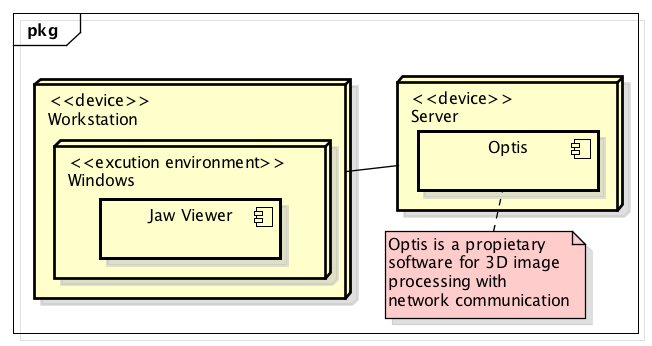
\includegraphics[width=0.5\textwidth]{deployment_diagram}
	\caption{Deployment Diagram}
\end{figure}

\subsubsubsection{Component Diagram} 

The Jaw Viewer is built with three components:

\begin{figure}[h!]
	\centering
	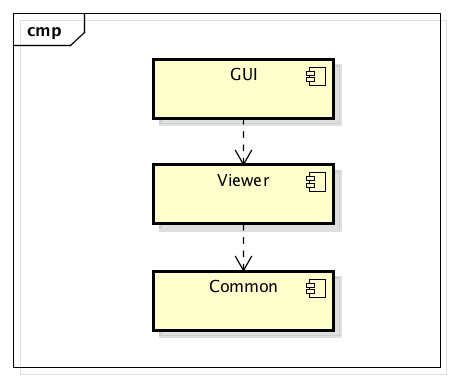
\includegraphics[width=0.4\textwidth]{component_diagram}
	\caption{Component Diagram}
\end{figure}


\subsubsubsection{Domain Model}

\begin{figure}[h!]
	\centering
	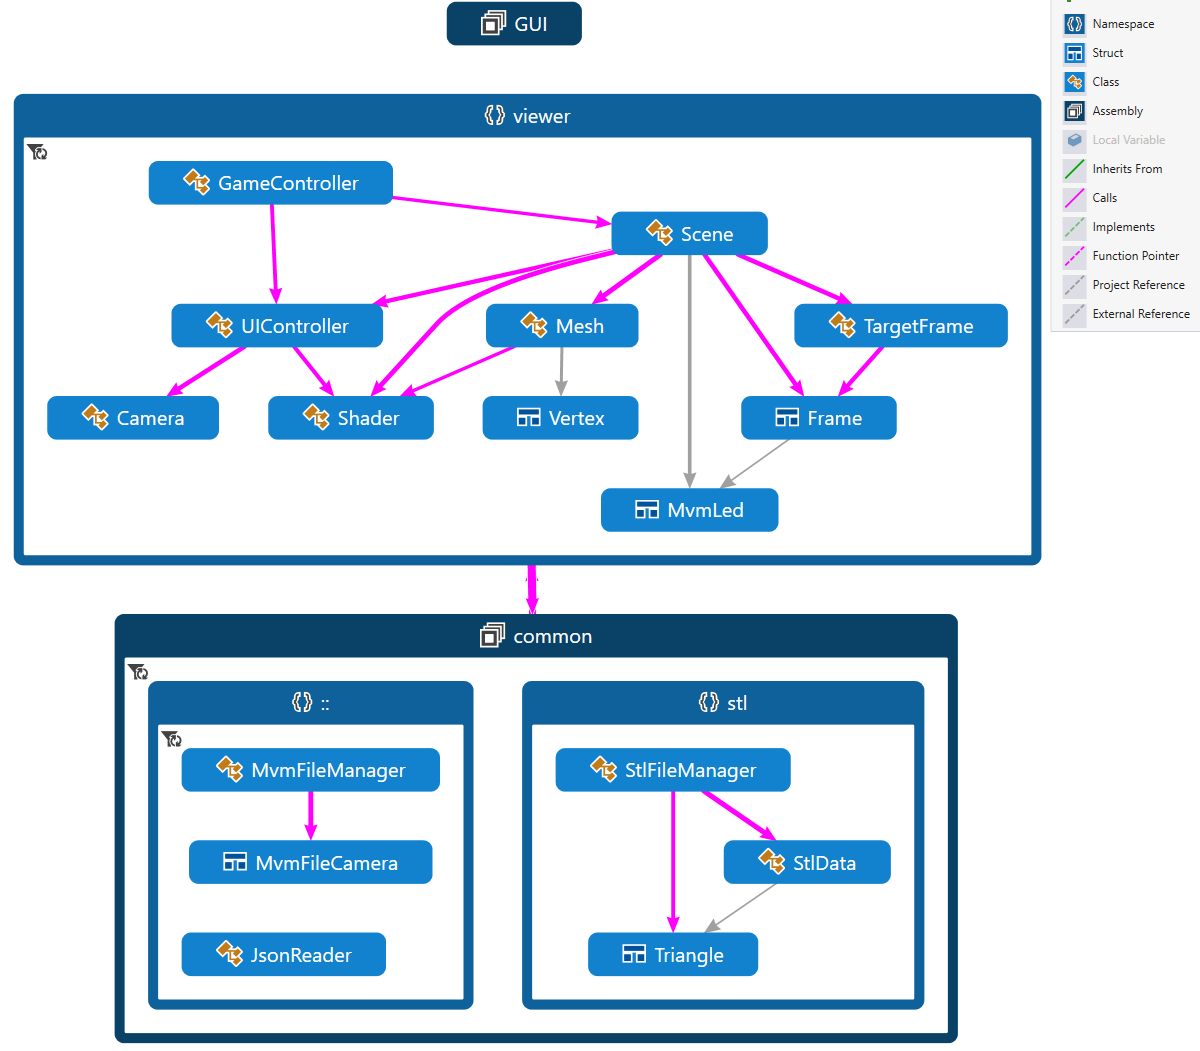
\includegraphics[width=1\textwidth]{domain_model}
	\caption{Domain Model}
\end{figure}

The Domain Model is divided in three parts, GUI, viewer and common. These build on each other hierarchically.

\paragraph{GUI} 
The GUI is a thin \verb|C#| client responsible of saving the user configurations and pass them to the viewer package in form of a \verb|json| file. It also contains the \gls{opengl} window (\verb|GLFWindow*|) as a child window of the main Window Form. The GUI starts also the \verb|C++| application.

\paragraph{viewer} Is the \verb|C++| application's core. It loads the configuration received from the GUI and uses the \gls{opengl} libraries to generate the 3D graphics displayed. It obtains the needed data from the common package.
The principal classes in the viewer package are:

\begin{itemize}
	\item[] \verb|Mesh|: A \gls{mesh} contains the \gls{vertex} data representing an \gls{anatomy}
	\item[] \verb|Scene|: Contains the \glspl{anatomy} or \glspl{mesh}, loading them from the \acrshort{STL} files and ordering them to render. It is also responsible of the initialization of the calculations needed for displaying the movement.	
	\item[] \verb|GameController|: Initializes the whole viewer package from the \verb|json| configuration and runs the game loop.
	\item[] \verb|UIController|: Contains the \verb|GLFWindow*|, registers the \verb|callback functions| used by \gls{opengl} to manage user input and directs this input to the \verb|Camera|.
\end{itemize}


\paragraph{common} Contains helper classes for reading the in \verb|json| saved configuration and parsing \acrshort{STL} and \acrshort{MVM} files containing the graphical and movement data.


\subsubsection{Development Environment} \label{tooling}


In this section we enumerate the technologies employed in the project and explain why we chose them.

\subsubsubsection{Technologies}

\paragraph{OpenGL} Graphic processing technology, for more detailed information check the glossary \gls{opengl} and the \ref{opengl} OpenGL section


\paragraph{Programming Languages: C++, C \#}

\paragraph{Integrated Development Environment (IDE): Visual Studio 2015}

\paragraph{Source Control Management (SCM): Git} 

\paragraph{Project Management Tool: Visual Studio Team Services \cite{visualstudioteamservices} } 

\subsubsubsection{Why these technologies}

\paragraph{OpenGL} \gls{opengl} is an obligatory technology as mentioned in \ref{term-reference:1} Terms of Reference.


\paragraph{Programming Languages:}
\begin{itemize}
	\item[] \textbf{C++:} \gls{opengl} is programmed in C++. Although none of us have experience in C++, we chose this language in order to avoid performance loses and maintain compatibility with the OpenGL libraries
	\item[] \textbf{C \#:} As Konrad H\"opli have experience with C \#, and in order to comply with the \ref{fr:1} FR 10, a modern GUI, we chose C \# for the Graphical Interface
\end{itemize}


\paragraph{Integrated Development Environment (IDE): Visual Studio 2015}
\noindent \\Both project developers have already worked with Visual Studio and the framework supports both C sharp and C++ programming languages. Visual Studio has also plugins which support \gls{glsl} syntax highlighting.

\paragraph{Source Control Management (SCM): Git} 
\noindent \\ Is also known by both developers, and is totally integrated in Visual Studio and in Visual Studio Team Services (see below).

\paragraph{Project Management Tool: Visual Studio Team Services \cite{visualstudioteamservices}}
\noindent \\ Is a cloud-based project management tool with a very easy setup and maintenance with which Konrad H\"opli works daily. The dashboard is clearly designed, allowing a clear view of the current tasks at a glance. All project members and client have access to the platform, which increases transparency. Among other services, it integrates Visual Studio and stores Git repositories.




